\subsection{Model improvements \label{sec:03_ModelImprovs}}


If the measured optics errors are known to be systematic the most natural
solution is to correct the machine model.
Multiple measurements need to be considered so the origins of the errors and
the applied corrections are unambiguous. The corrected model is than used to
recalculate the machine optics.

In CTF3 orbit response matrix (ORM), dispersion and finally phase space painting
measurements were compared with the model. Initially basically every section of 
the machine had pronounced some errors. In the following we discuss the
disagreements, list the most important corrections and the achieved accuracy.

Only in the last 2 years of the operations the phase space painting 
was employed, while previously the less accurate ORM method was used. 
The checks started with the ORM and dispersion data analysis scripts (MatLab)
which were comparing measurements with the model.
Initially different knobs were tried out to identify the sensitive elements.
The MatLab script were implementing functionality to automatically generate
MADX code to match the model to the measured data. For each corrector setting
corresponding MADX macro was generated followed by constraints
with the measured beam offsets for this setting.
%, for example:
%\begin{verbatim}
%  m03: macro =
%    { 
%       call, file=zerocorrs;
%       CR.IDHF0242 = 1.000000;
%       twiss, betx=10, bety=10; 
%    }; 
%  constraint, expr=table(twiss, CR.BPI0130, x) * 1000 = 0.000000;
%  constraint, expr=table(twiss, CR.BPM0155, x) * 1000 = 0.000000;
%  constraint, expr=table(twiss, CR.BPM0195, x) * 1000 = 0.000000;
%  constraint, expr=table(twiss, CR.BPI0208, x) * 1000 = 0.000000;
%  constraint, expr=table(twiss, CR.BPI0248, x) * 1000 = 0.320368;
%  constraint, expr=table(twiss, CR.BPI0275, x) * 1000 = 0.987091;
%  constraint, expr=table(twiss, CR.BPI0305, x) * 1000 = -1.080751;
%  constraint, expr=table(twiss, CR.BPI0395, x) * 1000 = -1.319713;
% constraint, expr=table(twiss, CR.BPI0425, x) * 1000 = 1.154727;
%  constraint, expr=table(twiss, CR.BPI0448, x) * 1000 = -0.348181;
%  constraint, expr=table(twiss, CR.BPI0475, x) * 1000 = -0.592727;
%  constraint, expr=table(twiss, CR.BPI0570, x) * 1000 = 1.293273;
%  constraint, expr=table(twiss, CR.BPI0610, x) * 1000 = -0.186182;
%  constraint, expr=table(twiss, CR.BPM0650, x) * 1000 = -3.322469;
%\end{verbatim}
The macros obtained for different optics measurements were combined together
and than parameters of interest fitted. Finally, the analysis of optics measurements 
ware repeated to obtain plots comparing the measurement with the modified model.

\subsubsection{Linac}

In the Linac ORM measurments agreed very well with the model. 
The only exception was around girders 5 and 6, where relatively small discrepancy was observed.
However, a simple correction of quadrupole strength fitting all the measurements could not be found.
Most probobly the error was due to imperfect modelling of travelling wave cavities at low energies,
in particular of the fringe focusing.
The modeling was quite uncertain because the effect depends on the exact geometry of the elements. 
It's worth mentioning that an improved algorithm in PTC [ref], 
which was used to model the Linac, reduced somewhat the discrepancy.
It was also not pursued in more detail because it did not pose any limitation 
for the beam performance. The beam was easily transported without any emittance growth to 
girder 10, where Twiss functions were measured using quad scan and than
corrected by rematching the linac optics from girder 6 to 10. The only drawback
was that rematching of girder 4 and 5 was not very accurate and eventually
needed several iterations, if it was needed.

\subsubsection{Stretching Chicane}
%
\begin{figure}[!h]
 \begin{center}
   \includegraphics[width=0.5\columnwidth]{fchicFringeFix.eps}
%  \subfloat[]  
%   {
%   } 
% \subfloat[]   
%   {\includegraphics[width=0.4\columnwidth]{.eps}}
 \end{center}
 \caption{Response measurement in CT line compared to the original and corrected model.}
 \label{fig:fchicFringeFix}
\end{figure}
%
The stretching chicane is composed of four bends and seven quadrupoles. 
Measurement with the quadrupoles switched off already showed large discrepancy in 
the vertical plane. Figure~\ref{fig:fchicFringeFix} illustrates an examplory measurement, 
where vertical corrector just in front the chicane was excited, compared to the model expectations. 
In the horizontal plane there was no expected focusing (the bends where of rectangular geometry) and 
the measurement fitted very well. 
The vertical focusing is due to the fringe fields and clearly the effect was overestimated by the model. 
Implementing the measured values of the magnet gap and the field integral reduced the descrepancy,
however, the best agreement was achieved when the field integrap parameter was increased by 80\%.
Very similar errors were found in CR and TL2. 

\subsubsection{Delay Loop}

The ORM measurements that were performed during initial years of 
the Delay Operation suffered from poor accuracy for several reasons. 
First, available aperture was very limited therefore relatively
small excitations could have been applied, otherwise they lead to lesses 
and therefore provided not reliable data. Secondly, the beam transport and 
orbit were sensitive to beam jitter. The pronounced beam energy drifts distorted
measurement in large dispersion locations. Later, SVD analysis of beam orbit
jitter pointed out not stable enough power supply of the septa magnets.
It was also discovered that injection septa had $4~mrad$ roll error, 
what made the vertical steering difficult but also translated the jitters 
into the vertical plane.
Finally, the BPI's in DL suffered from beam position dependent droop that 
was introducing yet another error in the orbit reconstruction. 

Hence, the signal to noise ratio of ORM measurement was bad and therefore 
a more robust method of Phase Space Painting was employed. 
In the meanwhile most of the problems were removed: septa were re-aligned,
beam energy drifts reduced by series of feed-back systems and the BPI droop
corrected independently for each electrode by a software program 
in the front-end computer.

Phase advance is the most accurate from all the optics properties measured
with Phase Space Painting. It is a model and BPM calibration independent measurement.
Therefore, it was the principal figure of merit in the model improvements. 
Naturally also dispersion measurements gave valuable intput.
The errors were not very large and in most of the cases they could be corrected with
Dispersion Target Steering.


Initially Phase Space Painting measurements were done using correctors in the injection
of the Delay Loop: \texttt{CT.DHD0495} and \texttt{CT.DHD0505} in horizontal
and \texttt{CT.DVD0495} and \texttt{CT.DVD0505} in vertical.
They had a drawback that the beam exiting DL was also affected and the model
had to take in into account. It was implemented, however, it made the measurement
less straight forward. Figure~\ref{fig:0302_PhSpPaint_DLini} shows 
the first measurements of phase advances in the Delay Loop compared with the model. 
The errors were very clear, however, there wer not linked to indiviudual elements. 
In order to get a better insight a few additional optics were measured: 
a weak one using only half of the available quadrupoles and 
variants of the nominal one with corrections incorporated.

The situation could be improved by adjusting edge focusing of the dipoles and septa.
However, a satisfactory agreement between the model and 
all the available measurements was never reached. 
It was than understood that the very optics, 
particularly in the vertical plane, was extremely sensitive to the initial conditions,
beam energy and orbit. For example, only a few milimiter orbit distortion 
in the horizontal plane gave rise to 100\% beta beating. 

\begin{figure}
 \begin{center}
 \subfloat[]
   {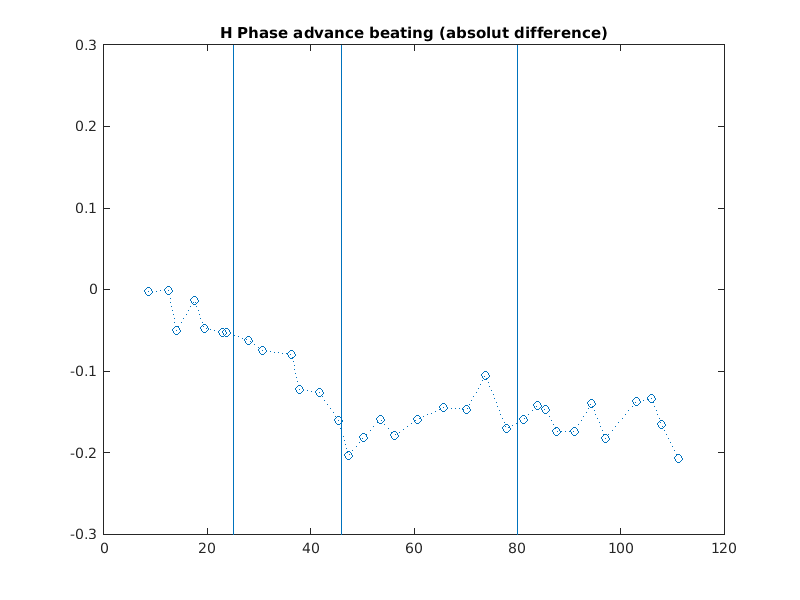
\includegraphics[width=0.49\columnwidth]{PhSP7364974395_PHASEbeating.png}}
 \subfloat[]
   {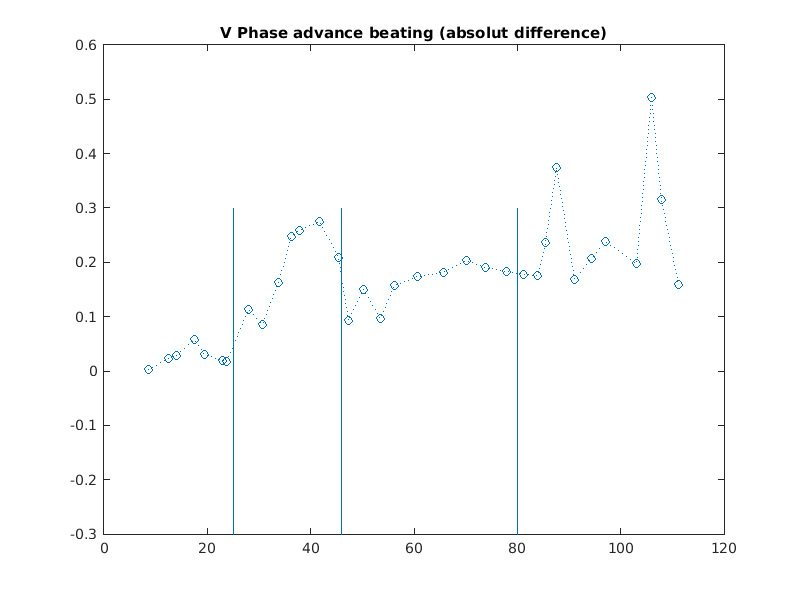
\includegraphics[width=0.49\columnwidth]{PhSP7364974508_PHASEbeating.png}}
 \caption{Difference of phase advance in the region of the Delay Loop}
  \label{fig:0302_PhSpPaint_DLini}

 \end{center}
\end{figure}


\subsubsection{TL1}

ORM measurements agreed with the model within error bar.
Phase Space Painting revealed that also here an issue with the edge focusing 
of the bends, although the correction had to be weaker compared to others sections 
presumable due to smaller bending angles in TL1 compared to CR and DL.


\subsubsection{Combiner Ring}

%Combiner ring posed an important issue during its first years of the operation. 
%Later it turned out to be related to instability induced by the RF deflectors
%[ref], but before this moment extensive set of ORM and dispersion measurements was done. 

To increase accuracy of the measurements in the CR circulating beam was observed for multiple turns. 
However, due to the fast decoherence of the large energy spread beam 
the oscillations were visible only over 3 turns. 
During the initial measurements the error was quite evident, however, not well localized.
Three of the four arcs had identical layout, including positions of 
the orbit correctors and the BPM's, so the measurements of these arcs 
could have been directly compared. As they showed the same response 
within the error bars, it was evident that the error is due to wrong parameters
of the magnets rather then powering errors or shorts in the coils.
%Thanks to the symmetry of CR it was easy to confirm absence of errors of particular magnets 
%as the responses of symmetric correctors were identical.
The discrepancies were traced to the already mentioned edge focusing of the bends and
a bug in the model where physical length of a J-type quadrupoles was in place 
of the one corresponding to the magnetic measurements. 
%Study of the on bench magnet measurements lead to conclusion that J type quadrupoles are in
%fact 7\% stronger than in the model because wrong magnetic length was used
%in the model. This brought a good agreement in the horizontal plane and in the dispersion. 
%Having experience with the error due to the edge focusing in the stretching chicane, 
%the FINT parameter was adjusted to match the measurement. 
The optics recalculated with the corrected model was 
much easier to establish the circulating beam and 
subsequent optics measurements (response matrix and dispersion) 
gave a satisfactory agreement with this model.


\subsubsection{TL2 and TL2 prime}

In TL2 the model corrections were much more difficult to determine because 
of the relatively complex layout.
Therefore, the response matrix measurements were done on several auxiliary optices
where different quadrupole groups were switched off~\cite{bib:Jack_PhD}. 
This way the edge focusing errors could be distinguished from 
quadrupolar errors and unambiguously determined. 
The best agreement was found when excitation constant for 
L-type quadrupoles was increased by 7\%. These devices were inherited from 
CELSIUS~\cite{bib:CelsiusMachine} and precise magnetic measurements were not available. 
Again, the optics reevaluated with the corrected model provided 
losless transmission and satisfactory agreement with the subsequent measurements.
